\documentclass[pdftex,10pt,a4paper]{article}
\title{\textbf{Experiment shopping list}}
\author{Ben Lambert}
\usepackage[authoryear]{natbib}
\usepackage[titletoc,toc]{appendix}
\usepackage[pdftex]{graphicx}
\usepackage{url,times}
\usepackage{graphicx}
\usepackage{epstopdf}
\usepackage{amsmath}
\usepackage[all]{xy}
\usepackage{pxfonts}
\usepackage{colortbl}
\usepackage{color}
\usepackage{subfigure}
\usepackage{gensymb}
\usepackage{ctable}
\usepackage[justification=centering]{caption}[2007/12/23]
\usepackage{longtable}
\usepackage{pst-func}
\usepackage{pst-math}
\setlength{\parindent}{0.0in}
\setlength{\parskip}{0.1in}
\usepackage[margin=0.5in]{geometry}
\renewcommand{\bibname}{Works Cited}
\usepackage{listings}
\usepackage{setspace}
\usepackage{algorithm}
\usepackage{bbm}

\newcommand{\HRule}{\rule{\linewidth}{0.5mm}}
\begin{document}

\maketitle
\doublespacing
\section{Introduction}
This document aims to provide a list of potential lab experiments which, if carried out, could elucidate the behaviour of tip and cap cells in the developing kidney. The purpose of this exercise is twofold: firstly to foster a better understanding of the mechanisms by which tip and cap cells move and proliferate; secondly to test \textit{in silico} simulations using the developed cellular automaton model against the results of \textit{in vitro/in vivo} experiments.

\section{Experiments}
\subsection{GDNF as a source of branching}
\subsubsection{Two explants}
The aim of this experiment is to determine conclusively whether branching occurs as a result of local maxima and minima in GDNF, by the examination of the branching patterns of two adjacent explants in culture. If GDNF concentration is an important factor for determining branching, we should see markedly less branching on the two sides of the kidney explant which are facing one another, as compared to the outer side. Furthermore, as we increase the concentration of GDNF this asymmetry between the two faces should be reduced, since there are sufficient levels of GDNF to saturate all Ret receptors, regardless of their geography. See figure \ref{fig:twoexplants} for a visual depiction of these potential outcomes. This experimental setup also should allow us to see the importance of the effect which nearby branches have on other branches, through effects other than consumption of GDNF. If there is reduced branching even after a saturation GDNF concentration is used then this might be seen as evidence for the moderating effects of nearby branches on other branches.

\begin{figure}[t] 
\centering
\scalebox{0.25} 
{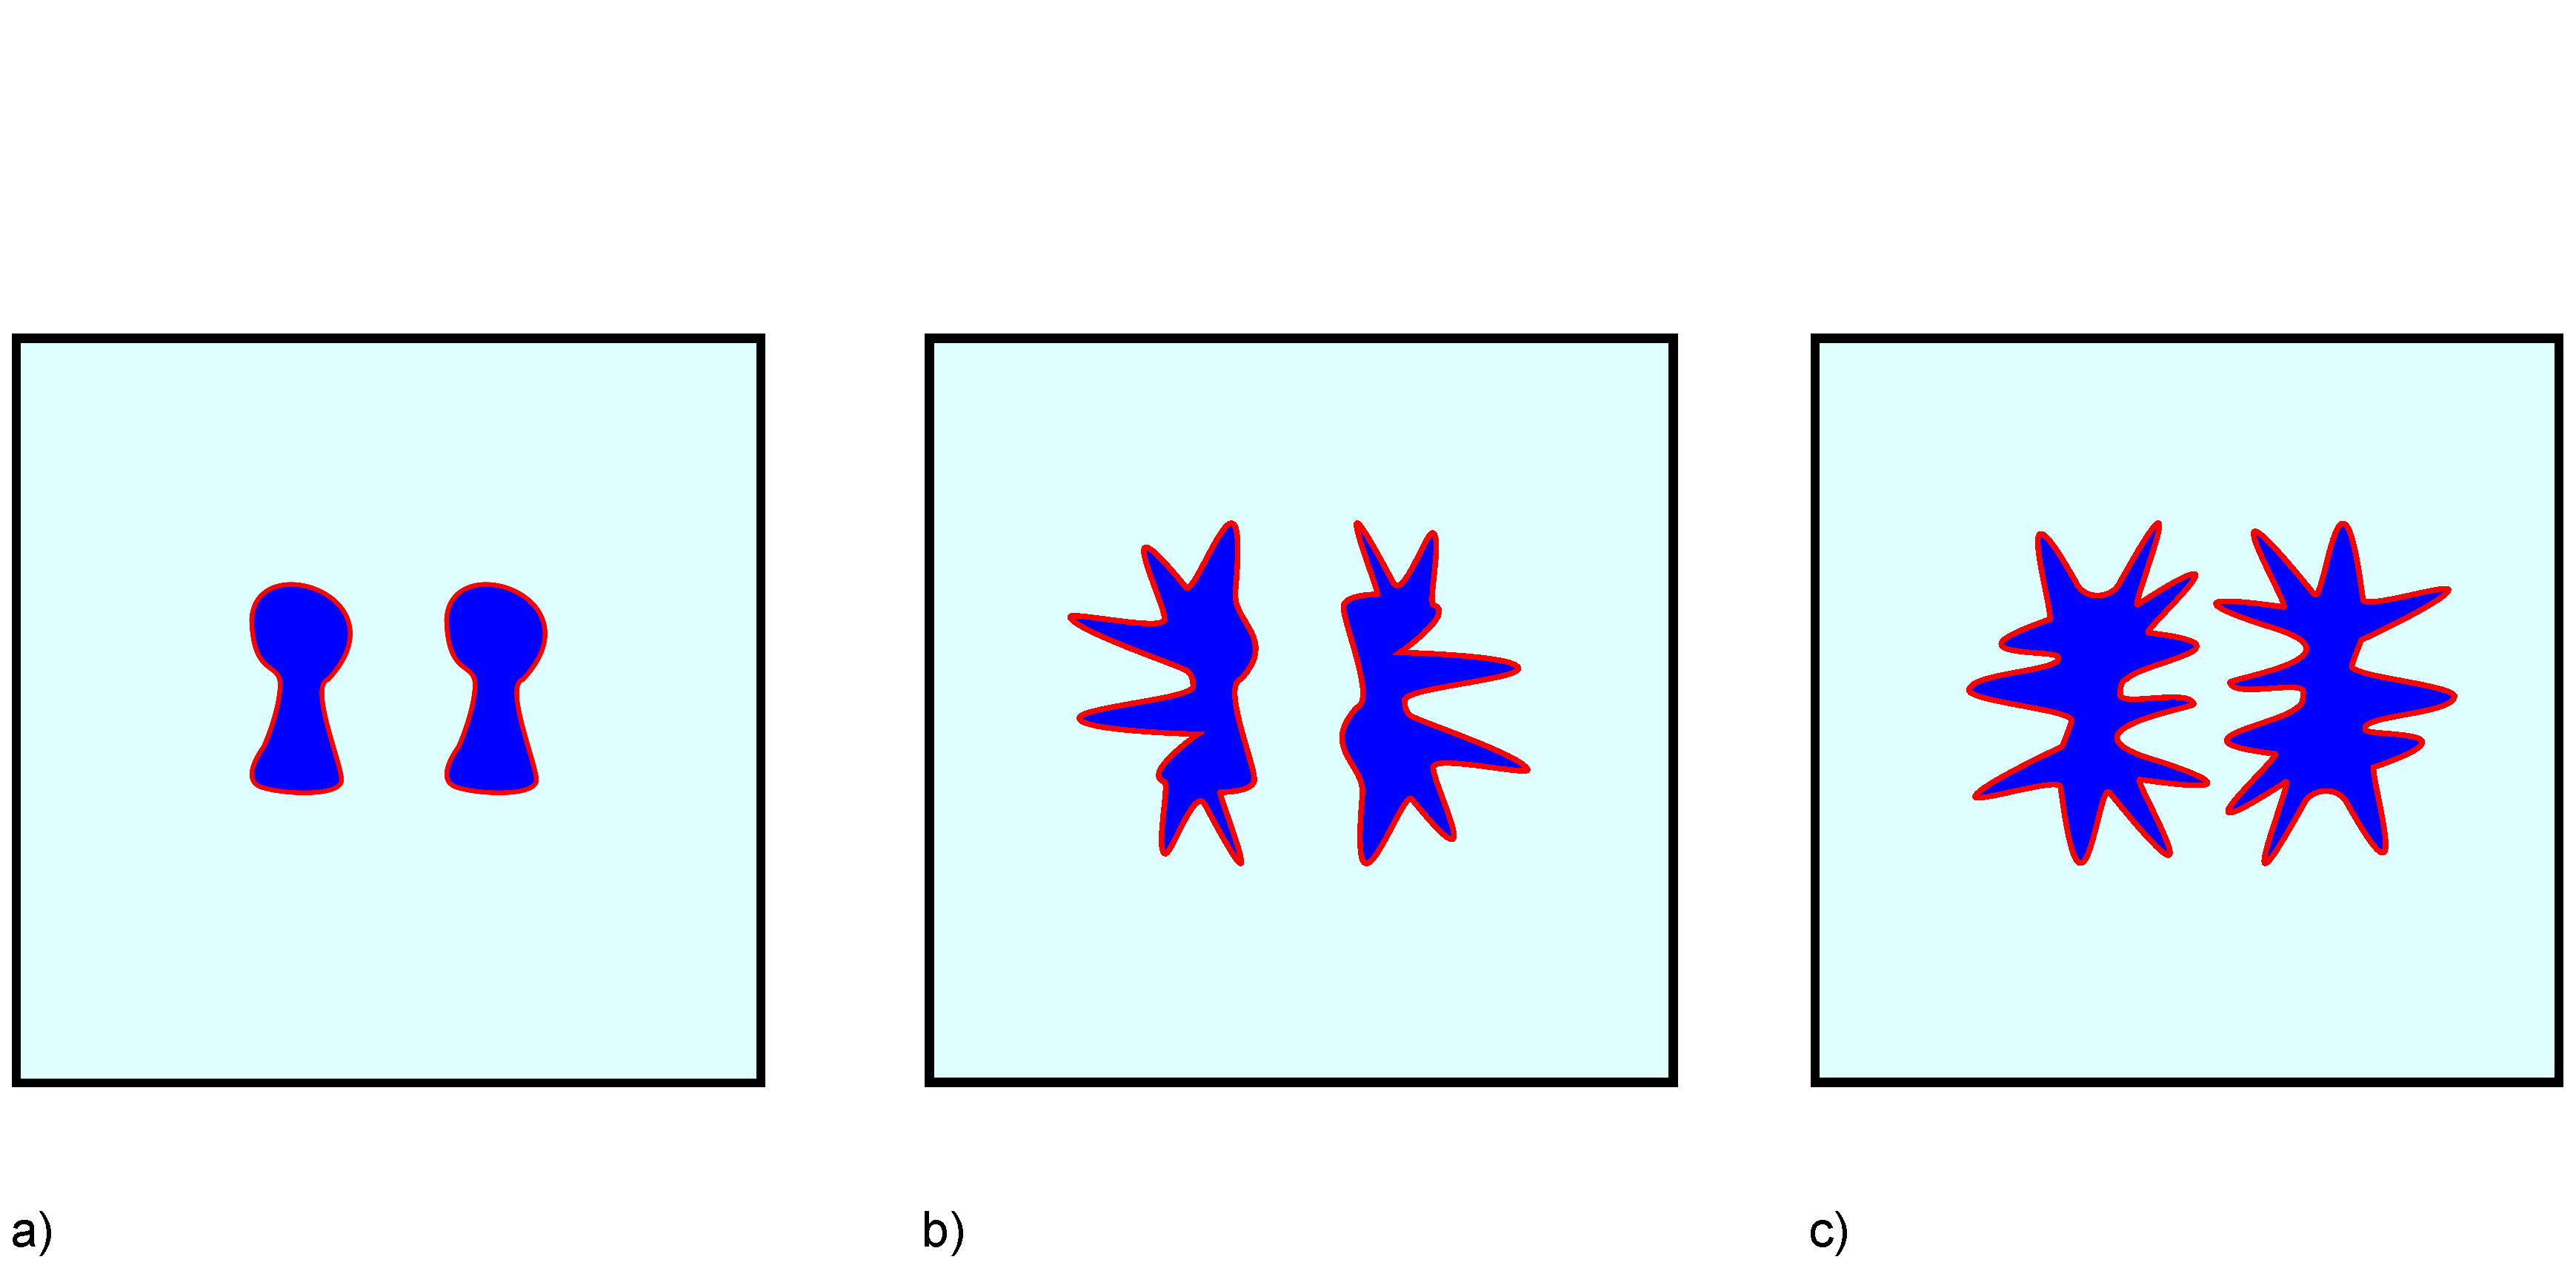
\includegraphics{experiments_1.eps}}
\caption{a) Shows the starting configuration of the proposed experiment, with the two explants adjacent to one another in a GDNF culture medium. b) Shows the morphology of the explants after the experiment has run for some time, with \textit{low} GDNF concentration being present in culture. c) Shows the same time point in an experiment where a \textit{high} concentration of GDNF has been used.}\label{fig:twoexplants}
\end{figure} 

\subsubsection{Two beads of GDNF}
This experiment looks at understanding whether local GDNF concentrations can be responsible for bifurcations in a mass of epithelium cells. The difference between this experiment and the two explants one above is that it removes the possibility that impaired branching is due to the interaction of the epithelium with the culture medium. By simply using beads soaked in GDNF this should allow for an environment which is more controlled (ie without the mechanical/other-than-GDNF chemical effects on other branches), and allow us to see whether there is evidence to support the claim that local concentrations of GDNF can cause tree bifurcations. See figure \ref{fig:twobeads} for a visual depiction of this experimental setup and a potential outcome.

\begin{figure}[t] 
\centering
\scalebox{0.25} 
{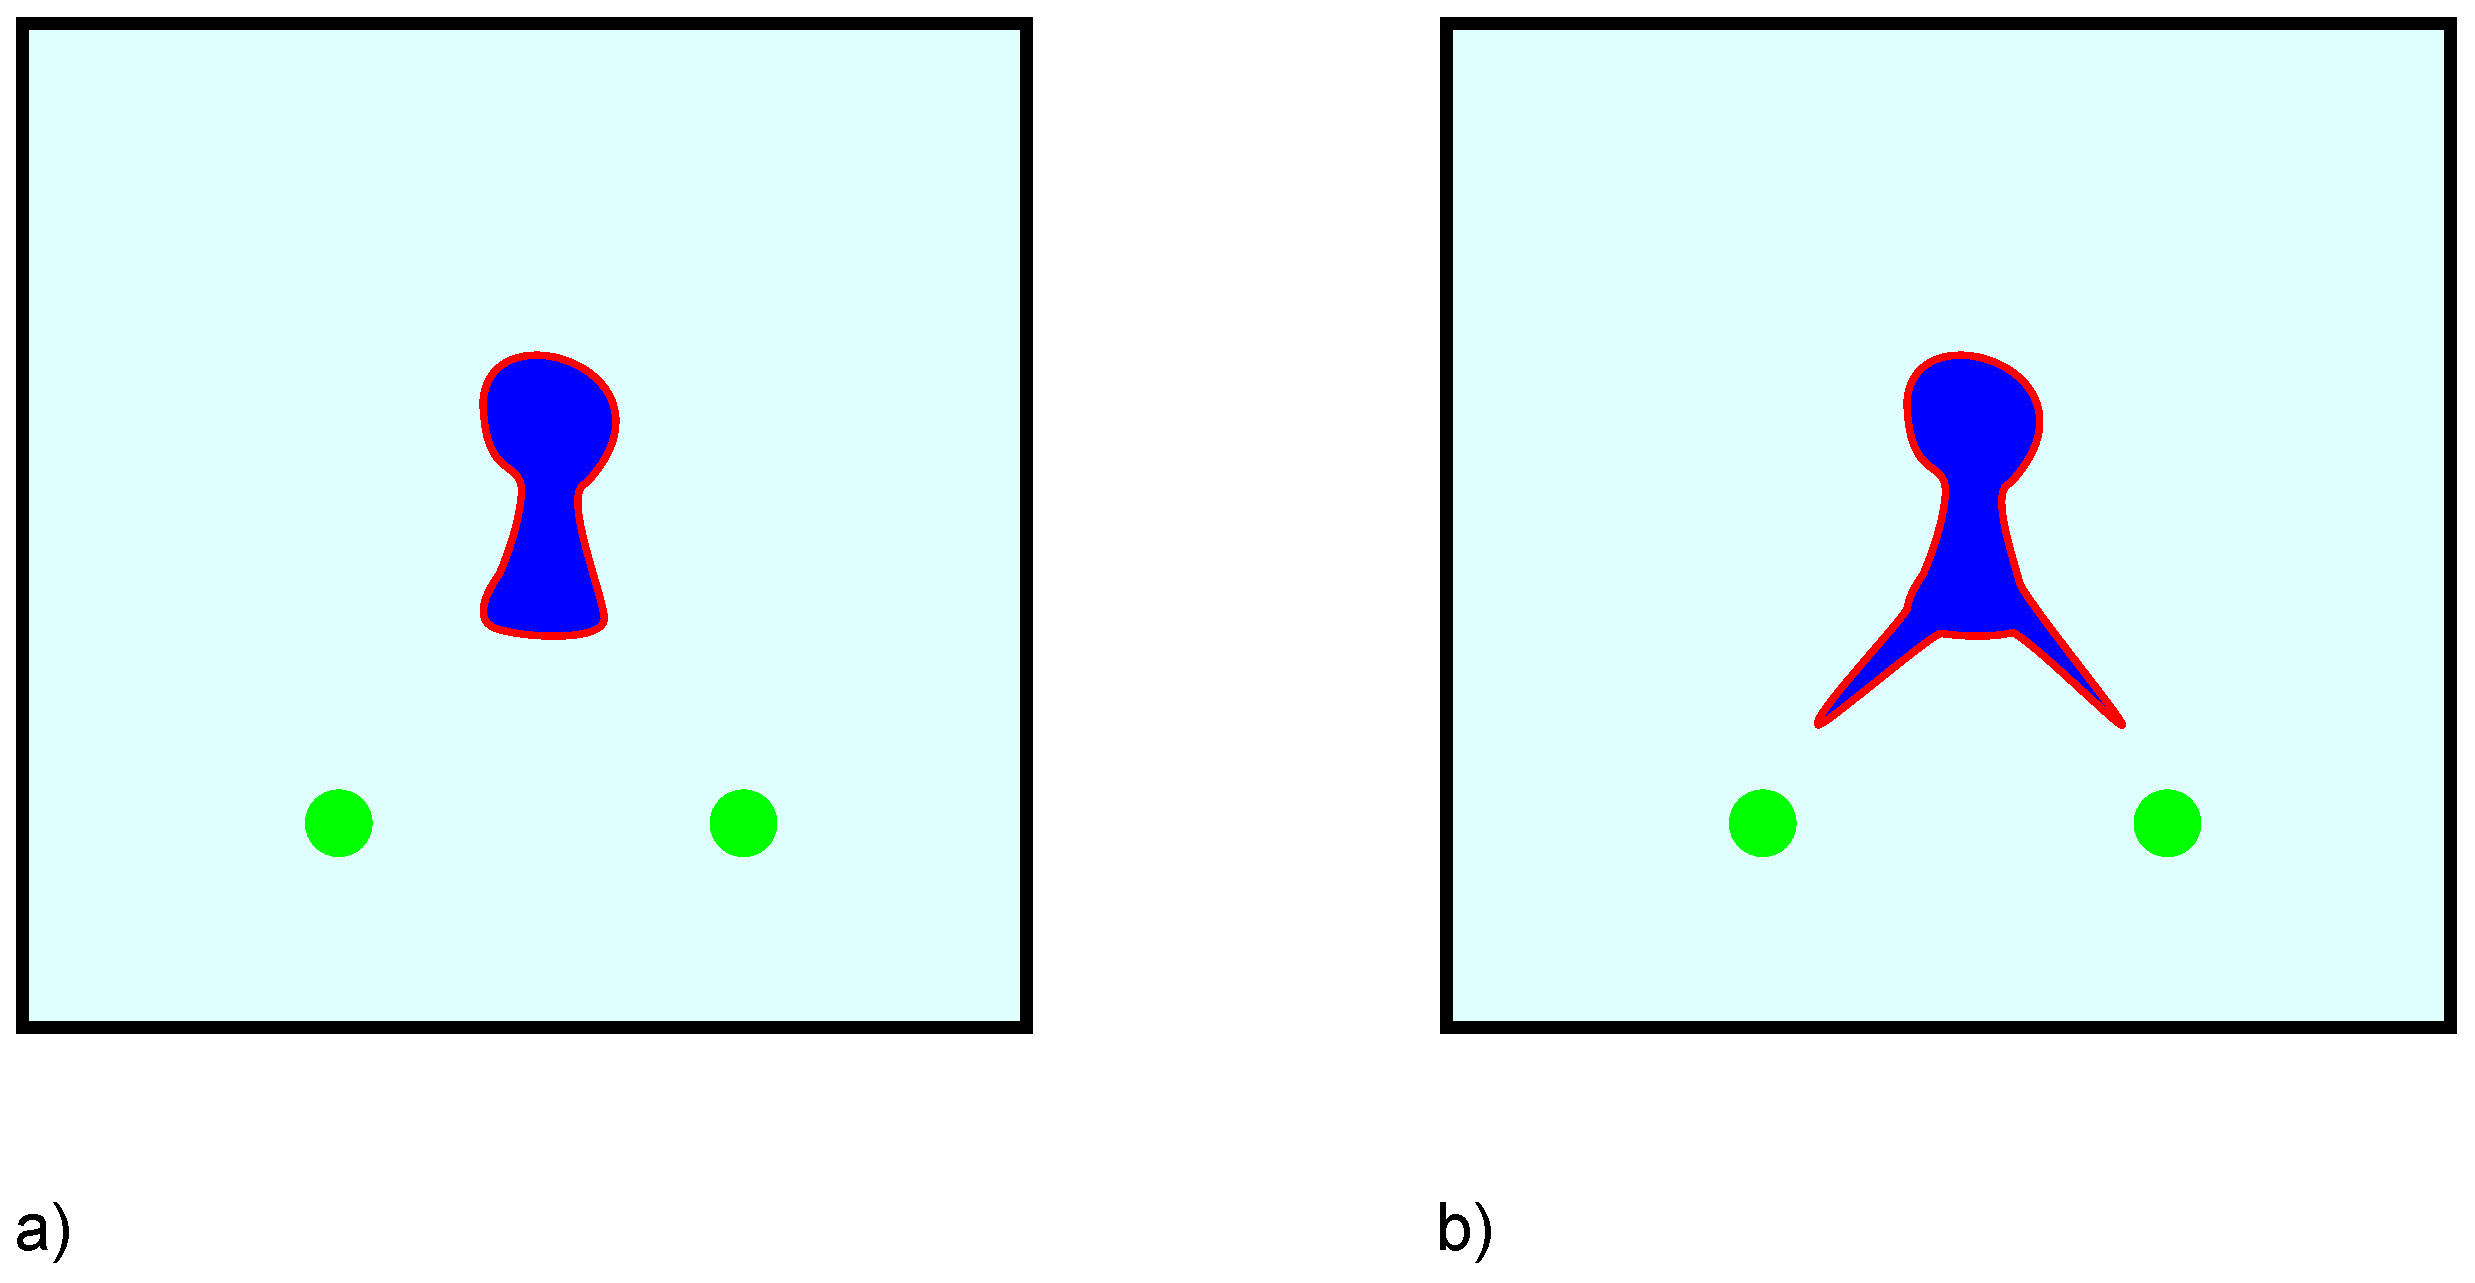
\includegraphics{experiments_2.eps}}
\caption{a) Shows the experimental setup with an explant (coloured blue with red edges), suspended in a medium bereft of GDNF apart from the two nearby beads (coloured green) that are soaked in GDNF. b) Shows how branching might occur in response to the local maxima in GDNF resulting from the bead point sources.} \label{fig:twobeads}
\end{figure} 

\subsection{Is the mesenchyme chemoattracted to the Uretic Bud or does it merely proliferate?}
\subsubsection{Isolated mesenchyme}
This experiment aims to investigate the relative importance of chemotaxis and epithelium-stimulated proliferation for the mesenchyme. Whereas it is likely that both of these mechanisms act, it is not clear which of these predominates in the developing kidney. Mesenchyme cells can be isolated from a developing kidney, and sustained if they are near a bead which has been soaked in BMP7 or FGF2 \cite{Dudley}.
The idea behind these experiments will be to look at the profile of mesenchyme cells after they are initially separated from an explanted Uretic Bud. In particular it would be interesting to look at how the mesenchyme population evolves in size and spatial organisation over time (if at all, since explants may lack an important chemoattractive/proliferative factor). I am not sure as to the viability of the experiment, both in terms of the practicality of keeping both mesenchyme and epithelium cells alive, as well as the required image-processing techniques to look at the spatial distribution of mesenchyme cells over time. However, if this experiment or something similar could be carried out, it could help to shed some light on the importance of chemoattraction vs proliferation for the mesenchyme. For a visual depiction as to how chemoattraction vs stimulated proliferation would differ in terms of results, see figure \ref{fig:messeparated}.

\begin{figure}[t] 
\centering
\scalebox{0.25} 
{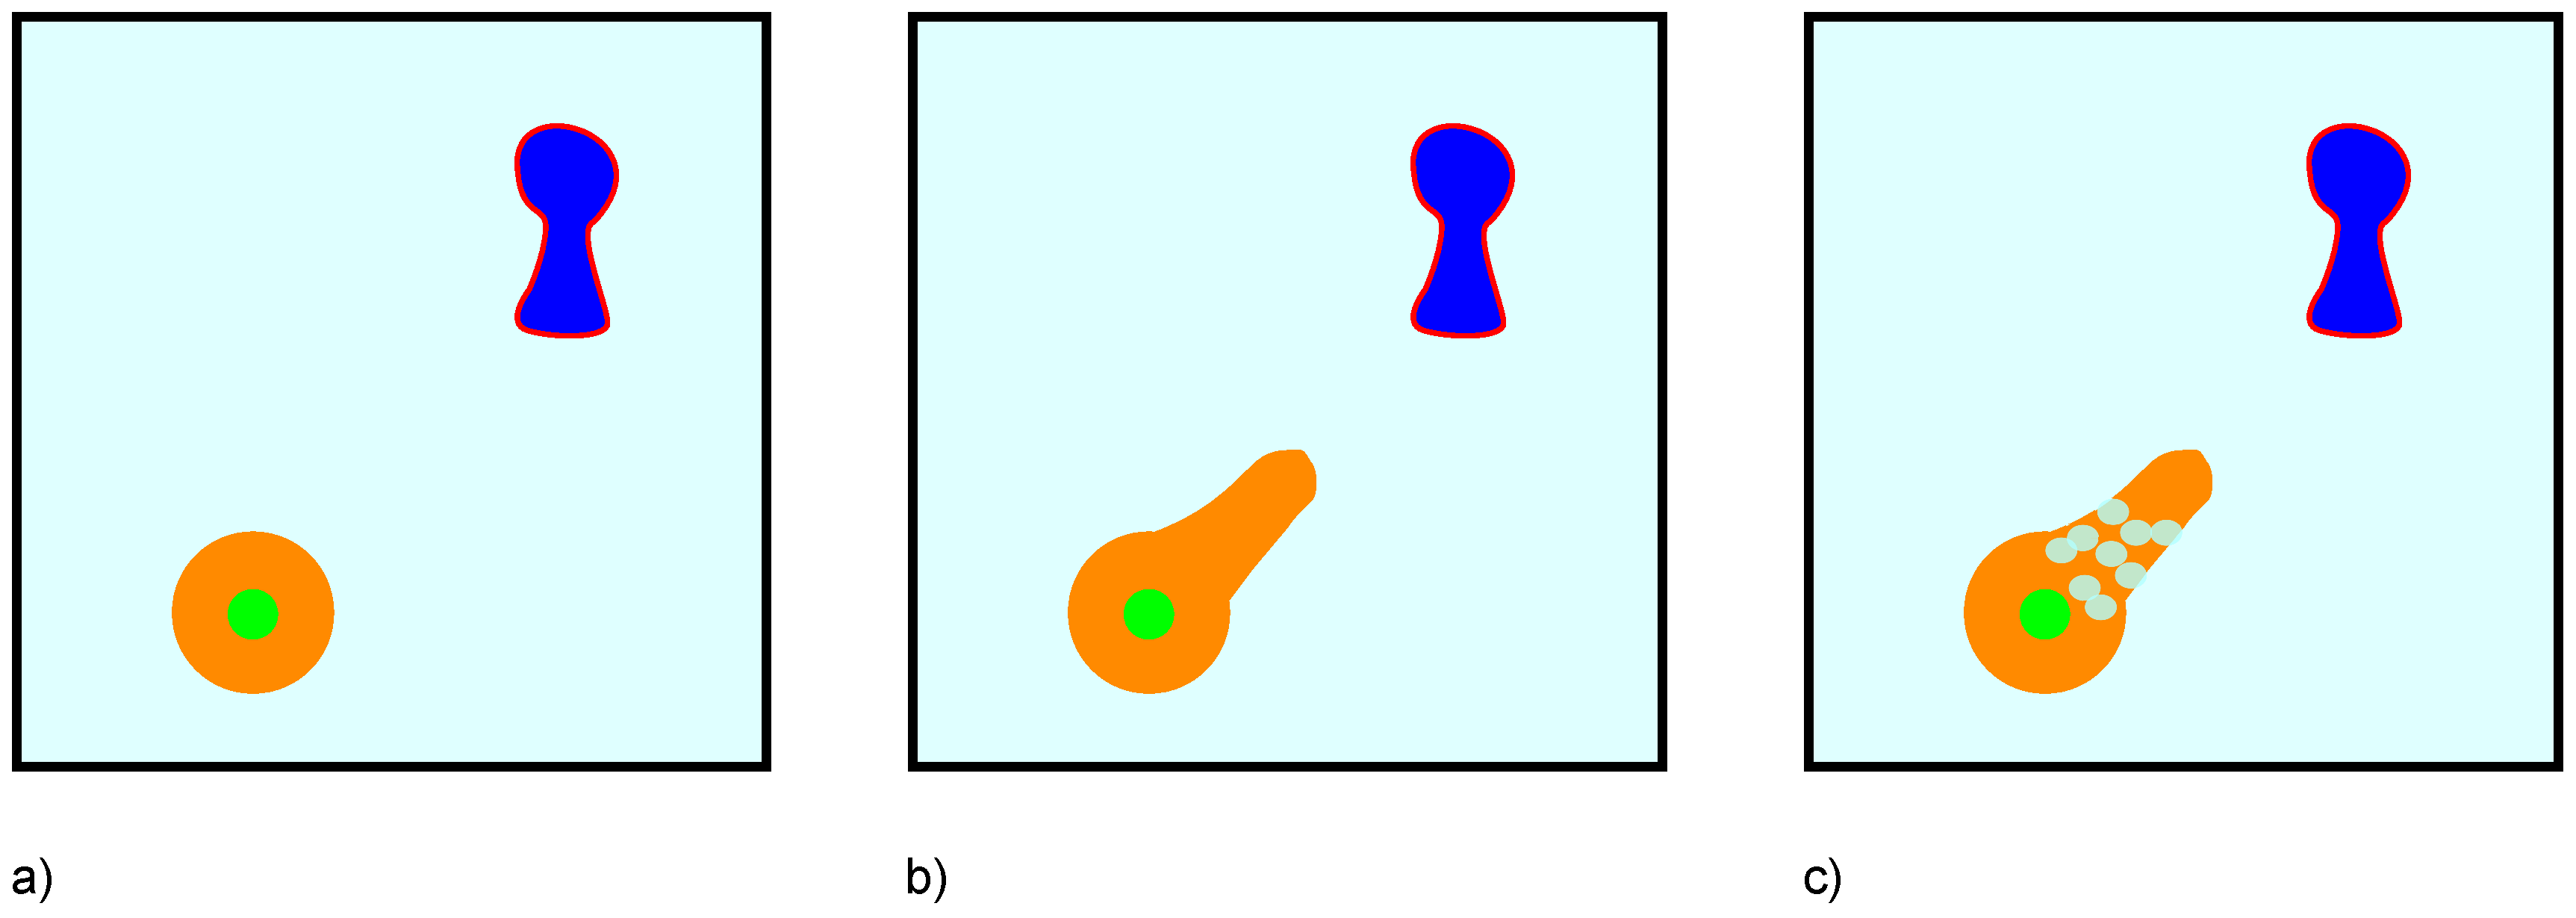
\includegraphics{experiment_3.eps}}
\caption{a) Shows the initial experimental setup with a bead of BMP7/FGF2 (in green) surrounded by mesenchyme (in orange), and a separate explant of epithelium cells. b) Shows how the distribution of mesenchyme might look after time if proliferation is the dominant mechanism. c) Depicts how the situation might look like if there was chemotaxis as well as proliferation. Note that each of these diagrams is stylised, as there would likely be growth of the UB out towards the mesenchyme.} \label{fig:messeparated}
\end{figure} 

\subsection{What is the difference between the trunk and the tip of the epithelium?}
\subsubsection{Redistribution of mesenchyme cells to the trunks}\label{sec:redistribution}
It is known that there are some differences between the phenotypes of the tip of the emergent Uretic Bud, due to differences in expression of Ret, as well as some other factors. However, it is not known whether these differences in the cells can be reversed; in other words do epithelium which have become one type of cell retain their relative \textit{pluripotency}? By explanting an emergent bud along with its adjacent mesenchyme cloud, it could be possible to design an experiment which tackles this question. If it is possible to separate the mesenchyme condensate and relocate from near the tips to being near the trunk, this would allow the experimenter to determine whether trunk cells retain an ability to proliferate in a manner which is distinct to tip cells (ie with daughter cells being produced in the lumen, and not remaining contiguous to their parent). If it would be possible to examine how the expression of Ret changes throughout the system as a whole this would also allow investigation as to whether this aspect of cell phenotype is fixed, or reversible dependent on GDNF concentration. Figure \ref{fig:tiptrunk} shows the how translating a mesenchyme cloud from the tip to the trunk region of the epithelium might cause growth if the cell changes were reversible.

\begin{figure}[t] 
\centering
\scalebox{0.25} 
{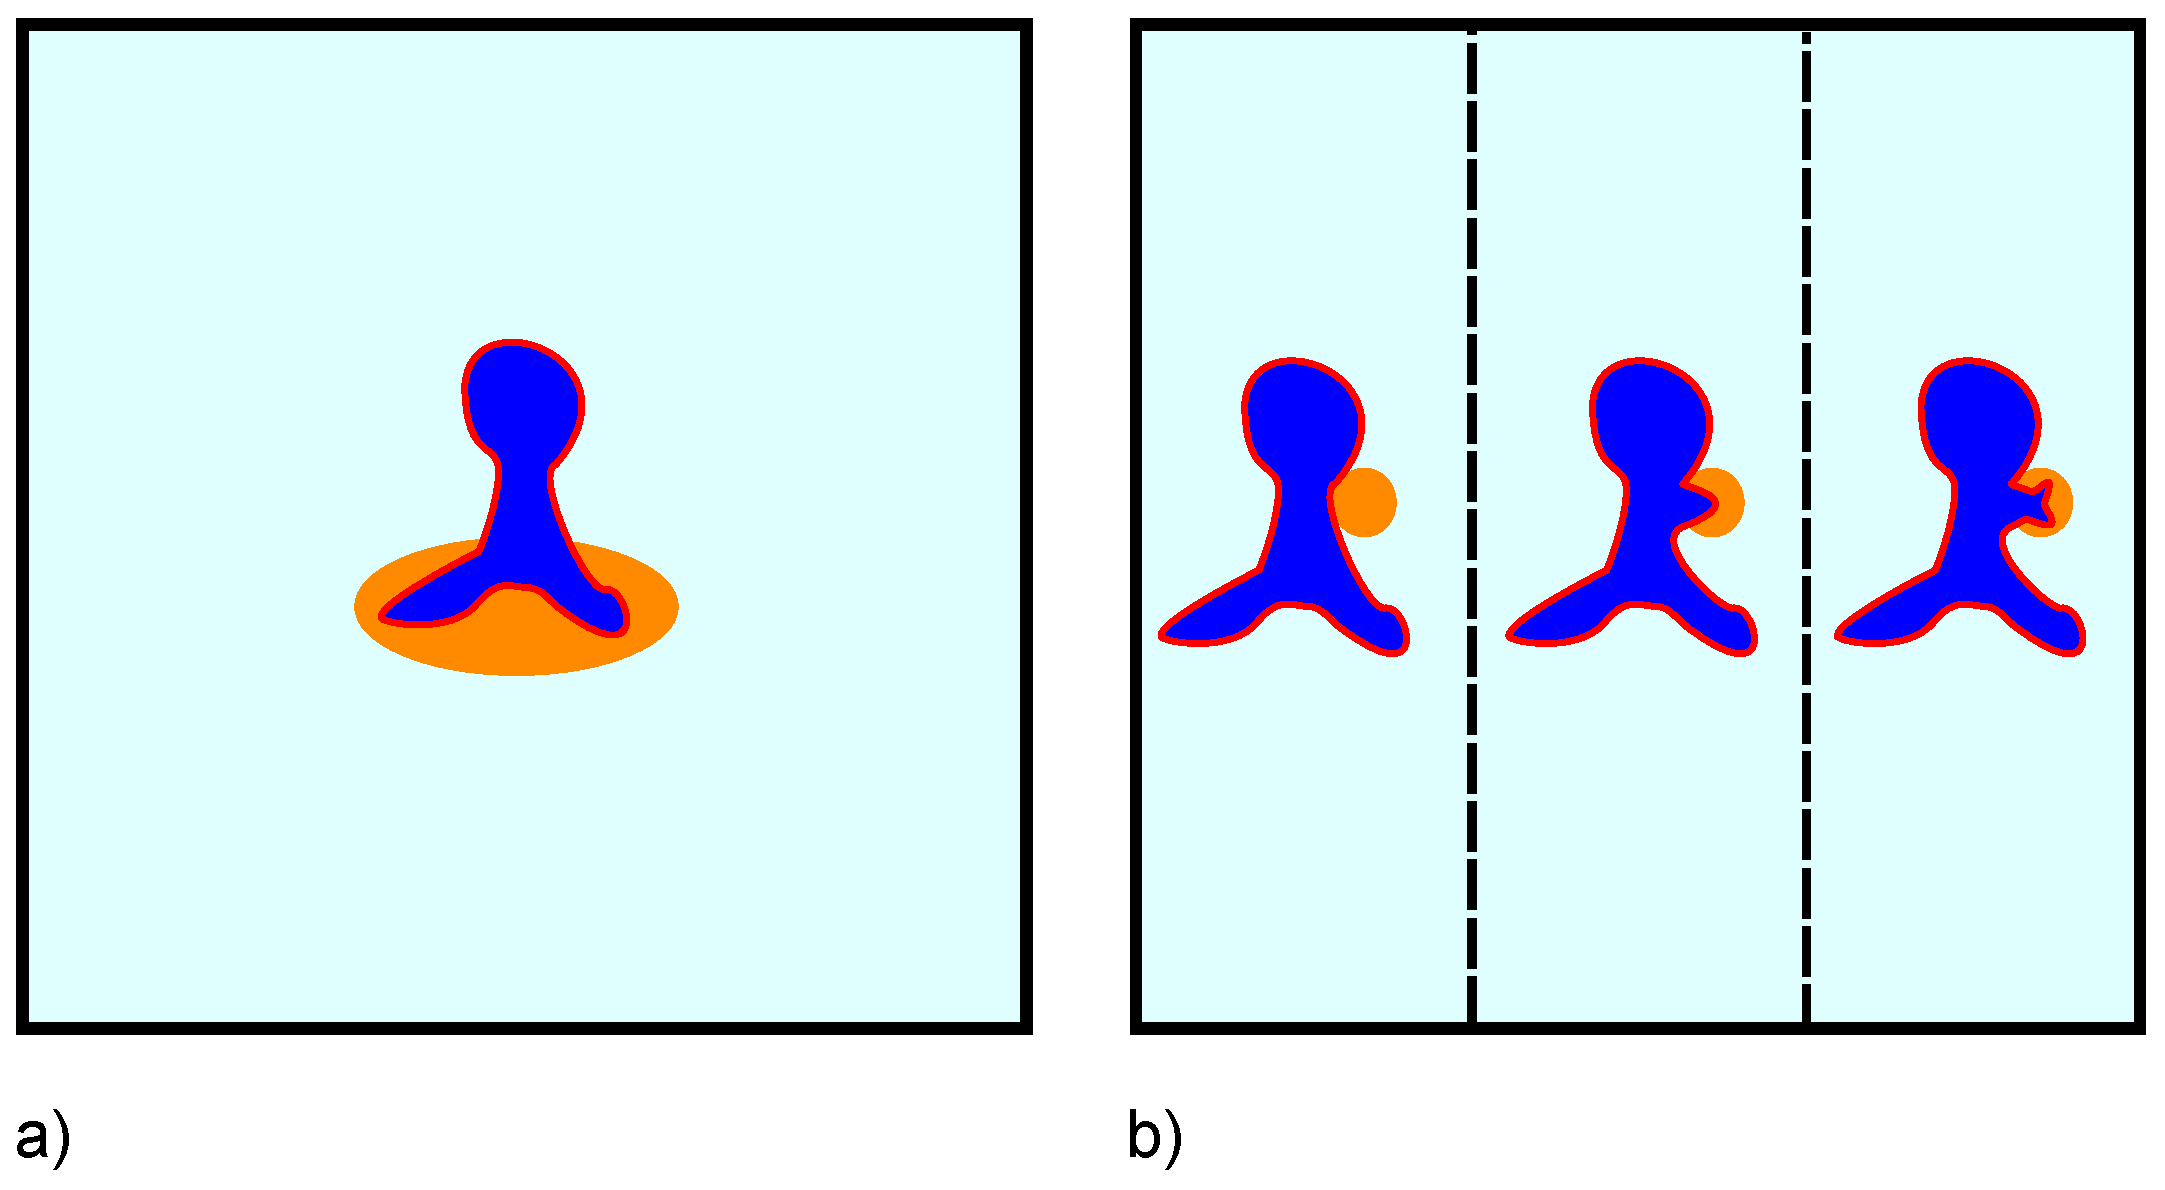
\includegraphics{experiments_4.eps}}
\caption{a) Shows the initial explanted UB with mesenchyme cloud. b) Shows how the epithelium may evolve over time if the cell types are reversible. The distribution of Ret expression throughout the epithelium would also potentially move from being highest at the tips to the trunks.} \label{fig:tiptrunk}
\end{figure} 

Another interesting aspect of this experiment would be that it could allow for a better understanding as to how mesenchyme is attracted to the epithelium. If it is attracted to the tips only (or less than the trunks), then (if the cell types remain fixed geograhically), it may be possible to visualise whether the mesenchyme migrates back up to the tips, or remains fixed.

\subsubsection{Tip or trunk cell only explants}
An issue with experiment \ref{sec:redistribution} is that it allows cells to migrate from the tip to trunk domains and vice versa. Hence the resultant patterning and Ret expression throughout the epithelium may not be indicative of cell pluripotency, but more reflective of the chemoattration of Ret-high cells (in the tip) towards the mesenchyme cloud. If either the tip or trunk region could be explanted singularly (without the presence of the other cell types), then this could allow for better understanding as to whether an epithelium's fate is sealed after its migration/creation in the tip or trunk. Here either an individual tip region or trunk region would be removed from an emergent UB, and placed adjacent to a cloud of mesenchyme. In both cases examination of Ret levels, as well as the resultant morphologies of epithelium should indicate the ability of cells to transition from one cell type to another.

\subsection{Changes to the initial distribution of mesenchyme and epithelium}
For benchmarking of the cellular automaton model developed it may be interesting for to investigate how changes in the initial distribution of mesenchyme or epithelium affects the branching which is witnessed. For the mesenchyme it would be interesting to see how the width and thickness of the mesenchyme affects the pattern of branching. As well as providing test cases to compare with \textit{in silico} simulations, it would also be informative as to how important the mechanical interaction between mesenchyme and epithelium is for generating particular morphologies. See figure \ref{fig:mesthickness} for a visual depiction of these experiments. In a similar vein it would be interesting (partly due to its implications for pathologically-developing kidneys) to investigate how branching is affected by removing a large section of the mesenchyme.

\begin{figure}[t] 
\centering
\scalebox{0.25} 
{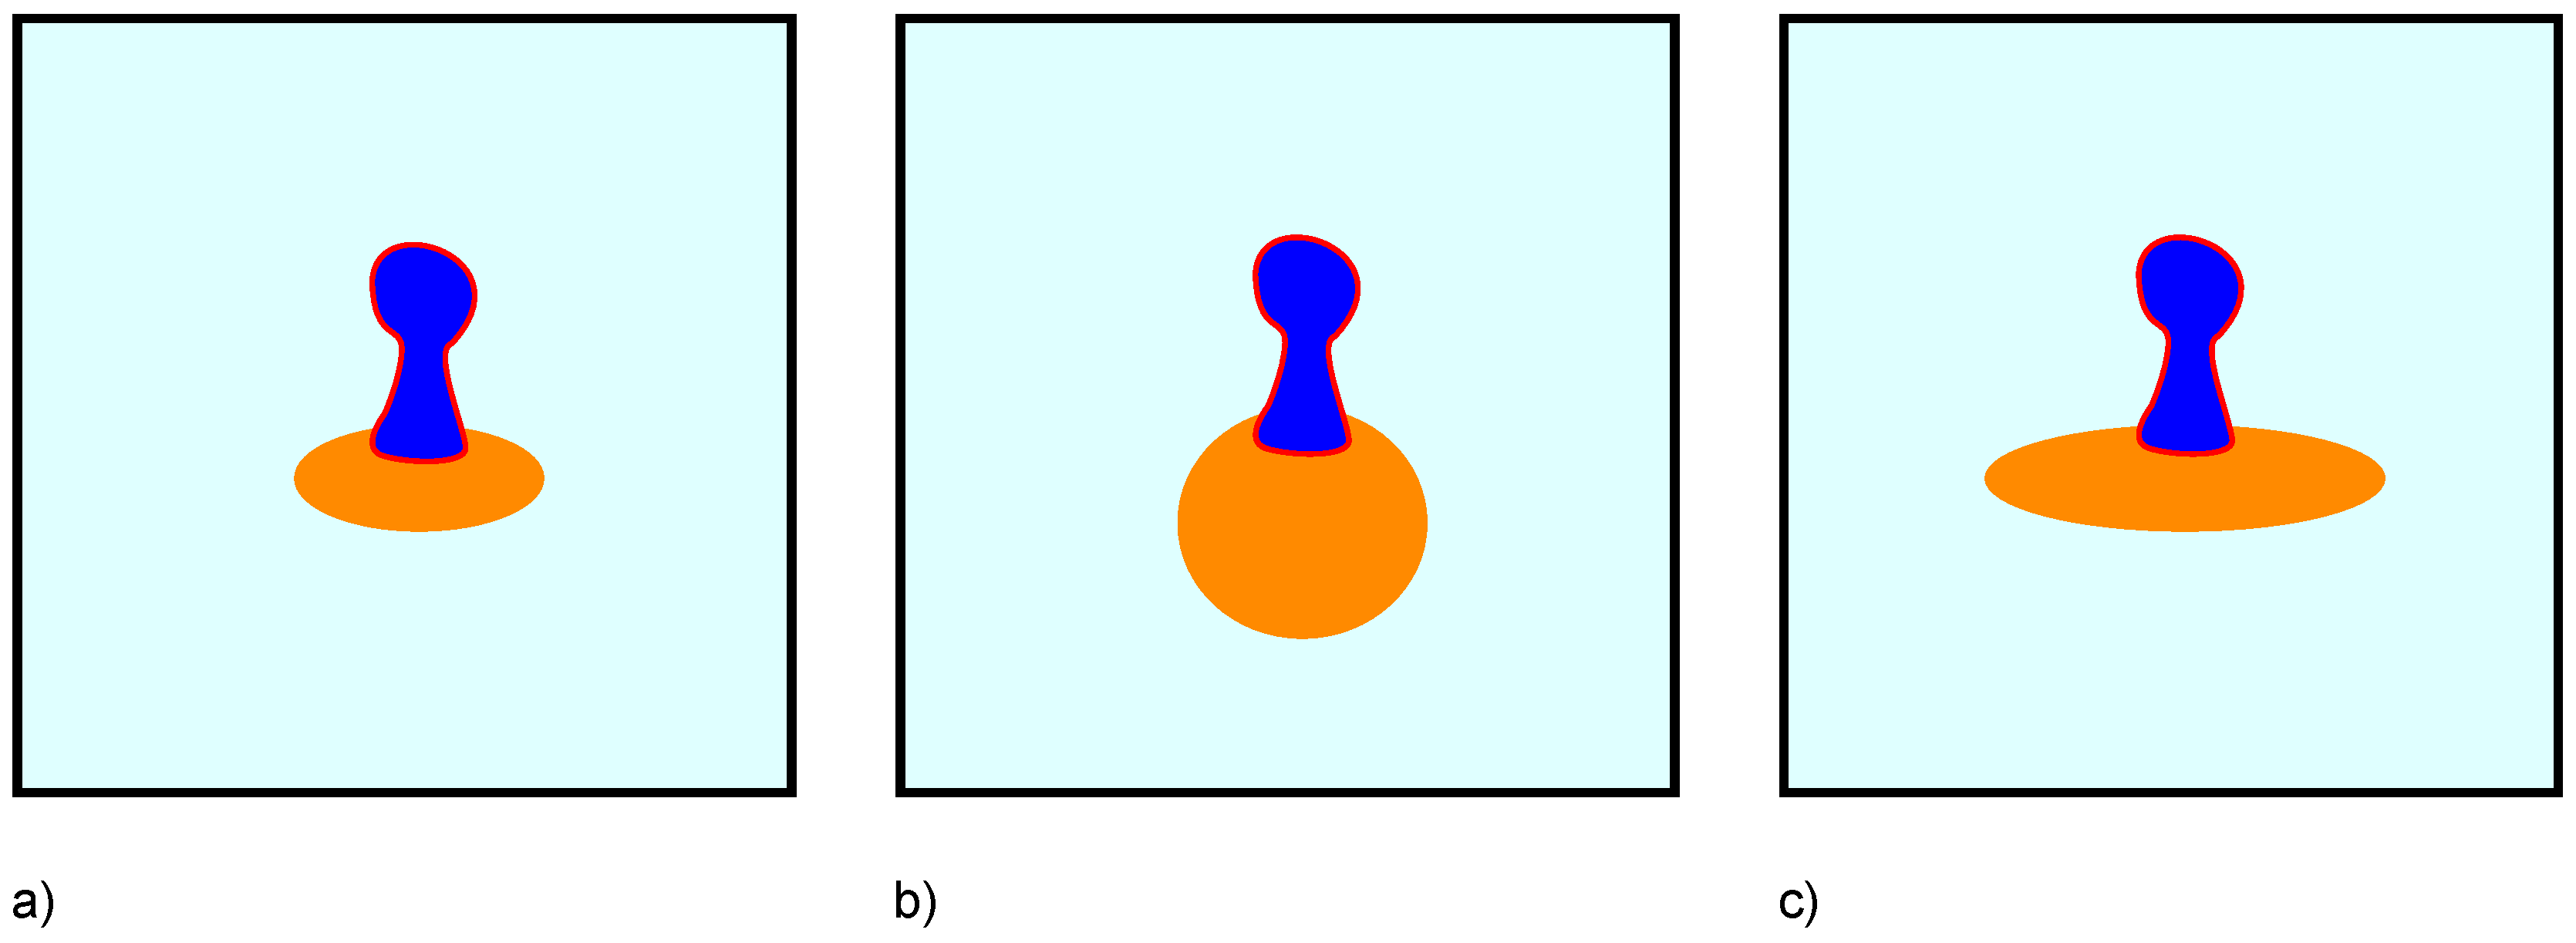
\includegraphics{experiments_5.eps}}
\caption{a) Shows the \textit{normal} initial condition for an explanted UB with surrounding mesenchyme condensate. b) and c) represent the initial condition of the UB after the mesenchyme condensate has been increased in depth and width respectively.} \label{fig:mesthickness}
\end{figure} 

It might also be a worthwhile experiment to investigate the effect of transplanting different parts of the mesenchyme, and seeing how these affect the pattern of growth induced in a UB. The reason for undertaking such an experiment would be to investigate whether the Six2-low mesenchyme cells retain their pluripotency, and ability to proliferate after they have become localised in an 'armpit' region of the branching epithelium. This region is normally where progenitors for Renal Vesicle cells form, after the mesenchyme undergoes a transition to epithelium.

It would also be interesting to investigate how 'slicing' off the first few layers of epithelium at the forefront of the UB affects future growth and branching. A comparison between this experiment and that where the mesenchyme is 'shocked', would provide experimental results that can be compared with \textit{in silico} simulations. It would also inform about the ability of the kidney to withstand shocks to one or another of the cellular compartments. It is not known whether these types of isolated shocks occur \textit{in natura} in response to outside stimuli. 

\subsection{'Straight' Uretic Bud emergence}
A particular feature of the \textit{in silico} simulations of the cellular automaton model which was indicated to be not observed in experiments was the 'bulging out' of emergent Uretic Bud tips after moving away from the Wolffian Duct. In reality the bud remains fairly 'straight-edged' in its path to the condensed cloud of mesenchyme. It was pointed out that the reasons for this could be because the ECM actually contains a factor which is important for limiting lateral growth of the epithelium from the bud. It would thus be interesting to investigate whether 'bulging' does occur if a nascent bud is removed, and placed in a medium containing only GDNF, or perhaps a separated cloud of mesenchyme. If it does not, then this may be indicative of the fact that there is not necessarily a separate factor which maintains the straight-edged bud, and may have a mechanical or another chemical (produced by mesenchyme or UB, but not by the ECM) explanation. See figure \ref{fig:straight} for a visual depiction of the 'straight' and 'bulging' Uretic Buds.

\begin{figure}[t] 
\centering
\scalebox{0.25} 
{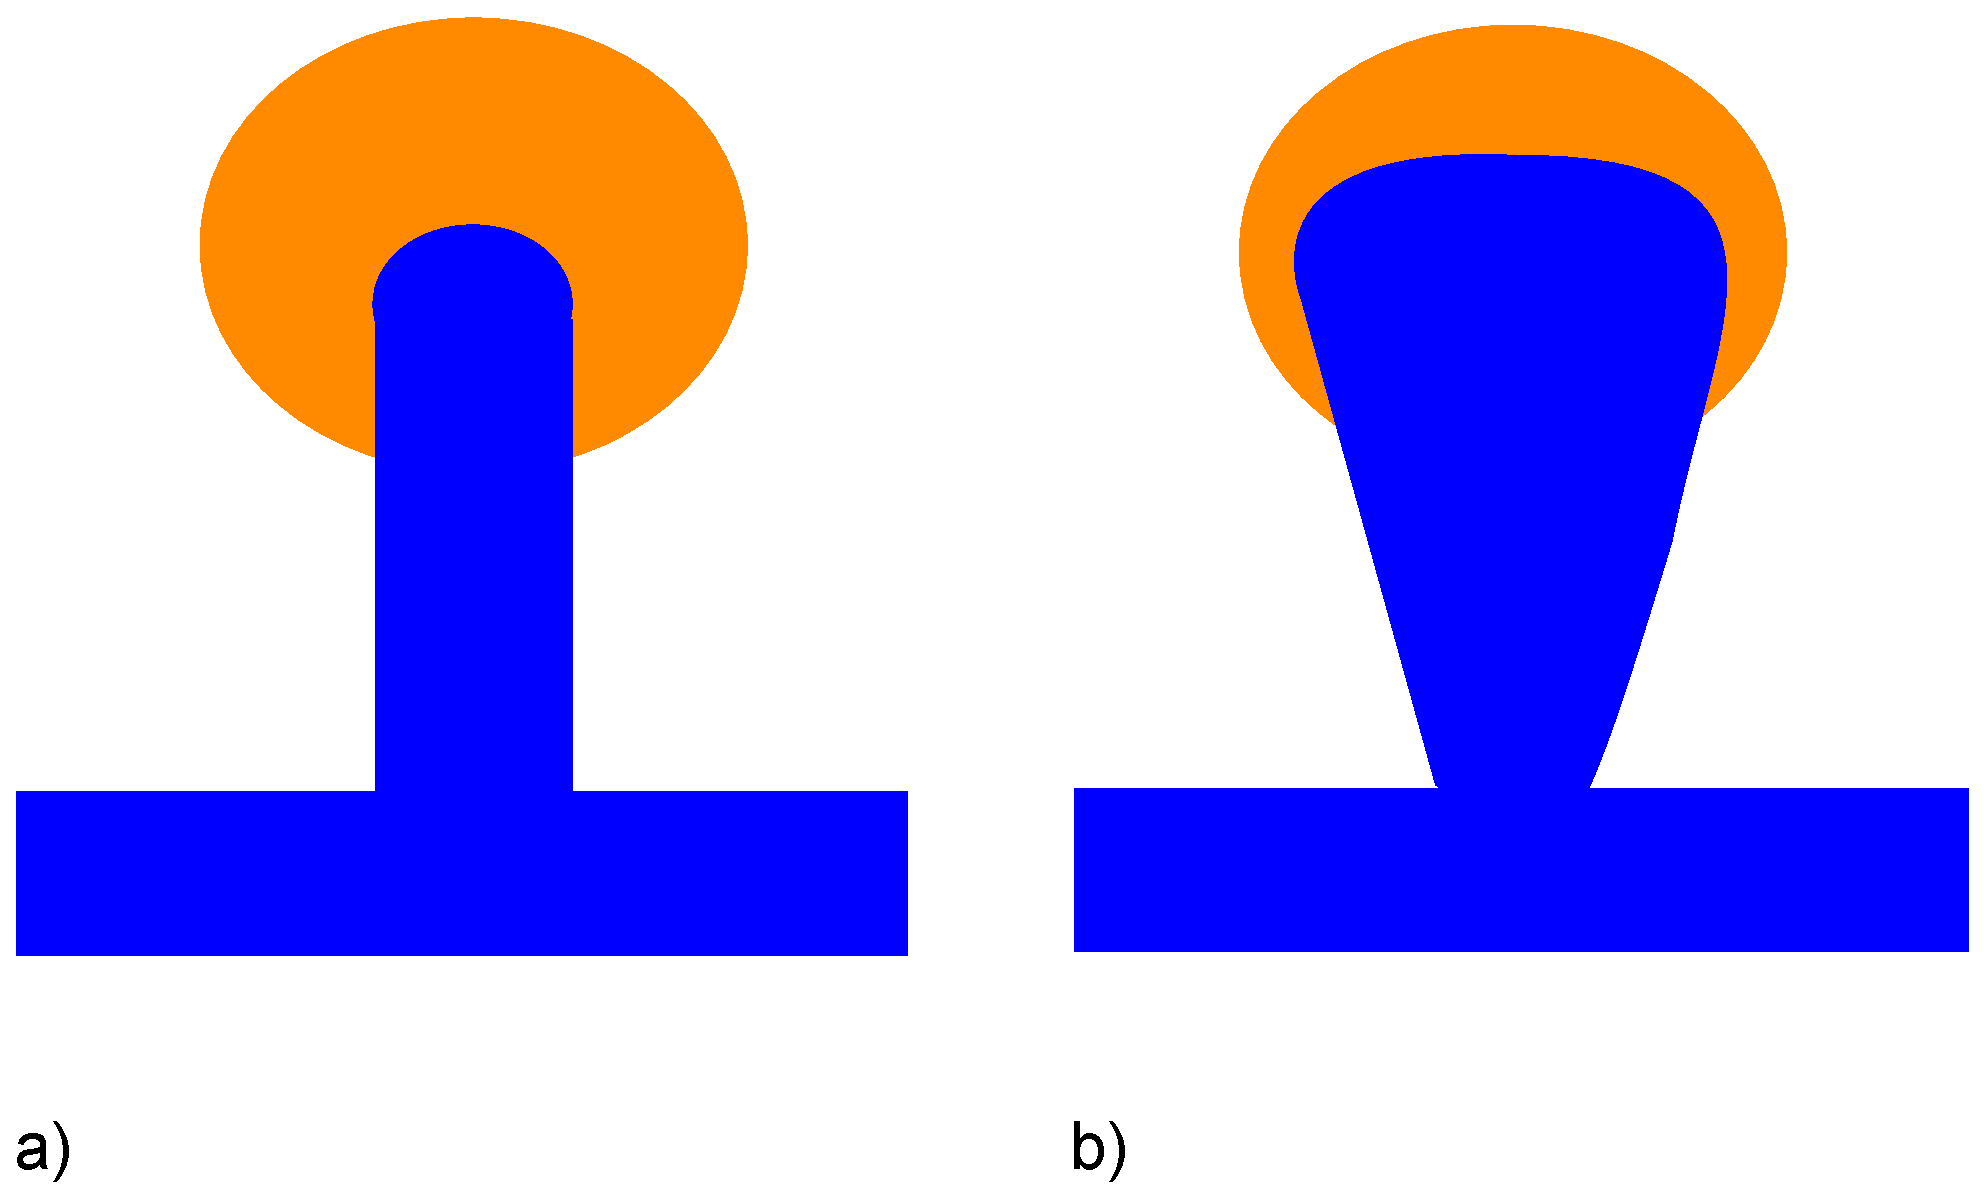
\includegraphics{experiments_6.eps}}
\caption{a) Shows the \textit{normal} emergence of a UB seen \textit{in vivo}. b) Depicts the emergence of a bud witnessed from \textit{in silico} simulations of the cellular automaton model developed.} \label{fig:straight}
\end{figure} 


\begin{thebibliography}{9}

\bibitem{Dudley}
Dudley, Andrew T and Godin, Robert E and Robertson, Elizabeth J.
\emph{Interaction between FGF and BMP signaling pathways regulates development of metanephric mesenchyme}. 1999, Genes and Development.
\end{thebibliography}

\end{document}